\documentclass[a4paper, punct,space,fancyhdr, fntef,UTF8]{ctexart}


\usepackage{szutils}%在这里放置需要的宏包,并设置部分所需内容
\usepackage{romannum}
\usepackage{zhlipsum}
\usepackage{booktabs}
\usepackage{multirow}
\usepackage[linesnumbered,ruled]{algorithm2e}

\setcounter{secnumdepth}{4}
\setCJKfamilyfont{kai}{全字庫正楷體}
\renewcommand{\kaishu}{\CJKfamily{kai}}

\begin{document}

	\pagestyle{empty}%不要页眉页脚
	%封面与诚信声明
	\include{data/cover}
	\include{data/statement}


	\zihao{-4}
	\tableofcontents%生成目录
	\thispagestyle{empty}%页脚不要页码
	%“目录”两个字的样式与section的样式一致,默认居中,故将设置section标题居左放置在生成目录后
	\ctexset{section={format=\Large\bfseries}}  %section标题居左

	%%%%正文开始,页脚有页码
	\cfoot{\zihao{-5}第 \ \thepage \ 页 \ 共 \ \pageref{lastpage} 页}%%%%lastpage为末页标签
	%正文
	\zihao{5}
	\pagenumbering{arabic}%页码使用阿拉伯数字
	\setcounter{page}{0}  %重新设置页码计数
	\pagestyle{fancy}

	\newpage


\centerline{\fangsong\bf\zihao{-2}{智能网联汽车GNSS位置欺骗攻击}}
\vspace{\baselineskip}
\centerline{\fangsong\bf\zihao{-2}{与功能安全危害联动预警策略设计及实现}}
\addcontentsline{toc}{section}{摘要(关键词)}%加入目录


\vskip 1cm

\begin{center}
	\kaishu
	\hspace{2cm}计算机与软件学院计算机科学与技术专业 \quad 李宇良
	\vspace{5bp}
	\newline
	学号:2018151004
\end{center}

\vskip 10bp

{
\kaishu
\hspace{5bp}{\zihao{-4}\textbf{【摘要】}}
随着机器学习、数据挖掘等技术的蓬勃发展,各种新兴技术也在不断产生。这其中就包括智能网联汽车。智能网联汽车区别于传统汽车,其搭载了各类传感器、执行器,同时结合了现代通信互联技术,可以实现车与车、车与人、车与路面等信息交换。然而,与智能网联汽车相关的GNSS位置欺骗问题也频频困扰各大厂商与研究者。因此,本文主要研究智能网联汽车上的GNSS位置欺骗攻击检测,以及相应的功能安全应急策略。本文的主要工作可以可概括为以下三点:
\begin{enumerate}
    \item 针对智能网联汽车上的GNSS位置欺骗攻击,基于机器学习中的LSTM网络,使用公开数据集建立训练集,设计并实现了一个可以有效实现攻击检测的算法。训练LSTM网络需要的数据为速度、转向角、向前加速度以及相邻时间戳之间车辆的移动距离。本文通过使用哈弗森大圆公式,将原始数据中的GNSS定位点数据转化为了距离。
    \item 在公开数据集上做一定的更改,得到欺骗数据集,并以此作为测试集进行了实验。实验结果表明,本文设计的算法可以有效检测到针对智能网联汽车的GNSS位置欺骗攻击。
    \item 依据ISO 26262标准,使用HARA方法对智能网联汽车在遭受GNSS位置欺骗攻击的情况下可能面临的功能安全风险进行了分析,同时划分了相应的风险等级,并设计了合适的应急策略。从而实现算法检测与应急策略的联动。
\end{enumerate}
综上所述,本文基于LSTM技术与ISO 26262标准,针对GNSS模块设计了位置欺骗攻击的检测算法,同时设计了对应的功能安全应急策略。检测算法可以有效工作,但在场景细化方面仍有提升空间。后续可以通过实车采集数据获得不同场景下的GNSS定位误差,从而细化不同驾驶场景中的检测表现。

\vskip 10bp

\hspace{5bp} {\zihao{-4}\textbf{【 关键词】}}
智能网联汽车;GNSS;功能安全;LSTM
}

    \section{引言}

\subsection{研究背景及意义}

\zhlipsum*[1-5]



\subsection{本文主要工作}

\zhlipsum[6-10,18][name=trad]



 
 第二章为推荐系统概览,并分类介绍了包括了基于内容、基于系统过滤与混合型推荐算法的一些典型的推荐学习算法。
 
 第三章为预备工作,首先简要回顾了Bayesian Personalized Ranking(BPR)推荐算法, 并对其局限性进行了一些探讨。
 
 第四章为适应性采样策略,主要研究了通过融合内容信息提出了适应性采样策略改进已有的均匀采样策略。
 
 第五章为整体的算法框架, 将适应性采样策略融入已有的BPR推荐模型。
 
 第六章为实验论证,主要内容为在适应性采样策略下的推荐算法的实验表现。
 
 第七章为结论与展望,首先简要总结了本文的一些工作,并对接下来进一步的研究工作做了展望。

	\section{相关技术简介}

\subsection{GNSS(全球卫星导航系统)概述}
全球卫星导航系统(Global Navigation Satellite System,下称GNSS),一般是指通过覆盖全球的导航卫星系统为地面或近地面用户提供全天候的三维空间坐标以及时间信息的无线定位系统。使用GNSS进行定位的用户可以通过具有GNSS信号接收器接收来自当前区域卫星的定位信号,并通过一系列的解码与计算得到较为准确的空间信息与时间信息,从而实现定位、导航、授时(PNT)的功能。

世界上第一个全球卫星导航系统是美国的GPS系统。该系统在设计之处一共由24颗卫星组成,其中21颗为工作卫星,3颗为备用卫星。而截至到目前,GPS系统的卫星数目已经达到了31颗。而在我国,第一颗北斗卫星在2007年4月14日发射,被在往后的若干年里不断完善北斗导航系统。截至2020年,北斗系统已经实现向全球提供服务的目标,与美国GPS、俄罗斯GLONASS、欧盟GALILEO并列成为四大全球定位系统。除了上述的全球性定位系统外,还包括区域系统和增强系统。其中区域系统有日本的QZSS和印度的IRNSS;增强系统则包括美国的WASS、日本的MSAS以及欧盟的EGNOS等。

GNSS的定位原理可以认为是求解一组方程。对于用户所处空间位置$(x_u, y_u, z_u)$,由于导航卫星所处的精确位置是可知的,同时卫星与用户之间的距离也可通过光速与时间差得到,因此可以列出以下方程组。
\begin{equation}
    \begin{cases}
        \rho_1=\sqrt{(x_1-x_u)^2+(y_1-y_u)^2+(z_1-z_u)^2}\\
        \rho_2=\sqrt{(x_2-x_u)^2+(y_2-y_u)^2+(z_2-z_u)^2}\\
        \rho_3=\sqrt{(x_3-x_u)^2+(y_3-y_u)^2+(z_3-z_u)^2}\\
    \end{cases}
    \label{eq:1}
\end{equation}
其中,$x_i$,$y_i$,$z_i$表示当前用于定位用户位置的第$i$颗卫星的空间位置。$\rho_i$则表示用户距离第$i$颗卫星的距离。求解上述方程组,即可求得用户位置坐标$(x_u,y_u,z_u)$。然而,在实际应用中,除了上述的三个未知数以外,往往还需要第四个未知数$t_u$作为修正项。原因在于,在计算用户位置与卫星间距离时,需要使用导航卫星中的原子钟与地面用户接收器的时钟作差得到钟差,但接收器的时钟精度要比原子钟精度低。这就导致最终得到的钟差会有一定的误差,因此需要加入修正项。此时的方程组为。
\begin{equation}
    \begin{cases}
        \rho_1=\sqrt{(x_1-x_u)^2+(y_1-y_u)^2+(z_1-z_u)^2}+ct_u\\
        \rho_2=\sqrt{(x_2-x_u)^2+(y_2-y_u)^2+(z_2-z_u)^2}+ct_u\\
        \rho_3=\sqrt{(x_3-x_u)^2+(y_3-y_u)^2+(z_3-z_u)^2}+ct_u\\
        \rho_4=\sqrt{(x_4-x_u)^2+(y_4-y_u)^2+(z_4-z_u)^2}+ct_u\\
    \end{cases}
    \label{eq:2}
\end{equation}
其中,$c$表示光速。
\subsection{GNSS位置欺骗攻击及检测方法概述}
目前,GNSS位置欺骗攻击还没有精确的定义。一般而言,“欺骗”是指某人或某程序利用数据篡改、数据伪造等手段成功伪装成另一个人或另一个程序,其目的往往是获取情报或影响被攻击者的正常运作。具体到GNSS位置欺骗攻击方面,攻击者会通过伪造错误定位信号或转发真实卫星信号等手段进行攻击。遭受欺骗攻击的GNSS接收器则会计算出一个错误的位置或错误的时间,从而导致依赖于GNSS定位的其他部件工作受阻或出错,甚至是无法工作。下面将对常见的GNSS位置欺骗攻击手段及检测方法进行简要介绍。
\subsubsection{欺骗方法概述}
\paragraph{基于信号模拟器的自主产生式攻击}

该攻击方式的主要思想是通过一个GNSS信号模拟器发送虚假GNSS定位信号来实现欺骗目的。目前,诸如Spirent公司的GSS8000等GNSS信号模拟器可以模拟出各种真实环境中的卫星定位信号。通过向接收机发送生成的定位信号的方法,可以实现一定程度上的位置欺骗攻击。但这种方法的缺点也很明显。由于GNSS信号模拟器所产生的信号是完全自主产生的,并没有与实际卫星进行信号同步,所以很容易导致接收机出现失锁或重捕的问题,从而导致欺骗被检测。另外,GNSS模拟器庞大的体积以及高昂的价格也是该欺骗方法的主要缺点之一。
\paragraph{基于接收机的接受产生式攻击}

该攻击方式所使用的干扰源主要由两部分组成,即接收机与信号模拟器。接受产生式攻击的基本工作原理与自主产生式攻击类似,都需要使用一个信号模拟器进行信号模拟生产。两者最大的不同在于,前者在产生虚假定位信号时所使用的参数由操作者或机器自身自主设置;而后者则是根据接收机接收到的真是卫星信号的估计结果,通过算法计算得到。与自主产生式攻击相比,接收产生式攻击所产生的信号与真实信号接近,其隐蔽性要更强。而其缺点在于,由于在使用真实卫星信号计算模拟参数时需要精确测定目标接收机与欺骗干扰源之间的三维位置关系,实现难度较大。尤其是当欺骗目标处于运动状态的时候,需要实时测定两者位置关系。也正因如此,这种欺骗手段一般只用于静止状态或低速运动状态下的目标。
\paragraph{基于信号转发器的转发式攻击}

我国在GNSS欺骗方面的研究主要集中在转发式攻击。该攻击手段所采用的思路与上述两种欺骗方法截然不同。该方法不再生成虚假信号,而是直接使用真实的卫星导航信号,通过使用转发器发射到目标区域,从而使目标接收到另一个空间位置的GNSS定位信号。与产生式攻击方法相比,该方法最大的优点在于不需要了解信号的内部细节(如GNSS信号格式、加密方式等),从而避免了大量技术细节与限制,并因此扩大了适用范围。而该方法的最大缺点在于,由于在信号转发时需要对原始信号放大,这会导致信号中的噪声被一起放大,从而导致转发信号与接收机接收到的真实定位信号在噪声水平上有较大的差别,容易被检测到。
\subsubsection{检测方法概述}
\paragraph{基于空间信息处理的检测方法}

该检测方法的主要思想是通过判别导航信号的空间信息来实现欺骗检测。具体来说,欺骗源的欺骗信号往往来自于
\paragraph{基于信号到达时间的检测方法}
\paragraph{基于机器学习的检测方法}


\subsection{LSTM概述}
\subsection{汽车功能安全概述}
\subsection{国内外研究现状}
\subsubsection{智能网联汽车GNSS位置欺骗攻击检测方面}
\subsubsection{基于预测的GNSS位置欺骗攻击检测算法}
\subsubsection{智能网联汽车GNSS功能安全方面}
\subsection{本章小结}

	\section{基于LSTM进行汽车位置预测的GNSS位置欺骗攻击检测算法}
\label{sec:chapter03}
\subsection{模型概述}
如\ref{sec:LSTM_gaishu}所述,LSTM作为传统RNN的改进模型,可以解决长序列问题中长期依赖的问题。对于本文中所涉及到的GNSS位置欺骗检测问题,由于汽车的移动轨迹可以看作是一个有依赖关系的连续序列,因此,可以使用LSTM作为问题的解决方案。模型的检测思路为,以被欺骗前目标车辆的CAN速度、IMU前向加速度以及转向角作为输入,输出为下一时刻目标车辆所处位置与当前车辆位置之间距离的预测值$dis_p$。计算$dis_p$与车辆实际移动距离$dis_g$的绝对值$dis_{abs}$,并设置欺骗阈值$\gamma$。若满足$dis_{abs}>\gamma$,则认为此时目标车辆受到了GNSS位置欺骗。$\gamma$的定义如下:
\begin{equation}
    \gamma=\epsilon_{GNSS}+\epsilon_{LSTM}
    \label{eq:gamma}
\end{equation}
其中,$\epsilon_{GNSS}$表示汽车GNSS模块定位误差,$\epsilon_{LSTM}$表示检测模型的预测误差。
本文所使用的模型结构包括输入层、包含50个神经元的隐藏层以及输出层。如图\ref{fig:my_model_arch}所示。
\begin{figure}[htbp]
    \begin{center}
        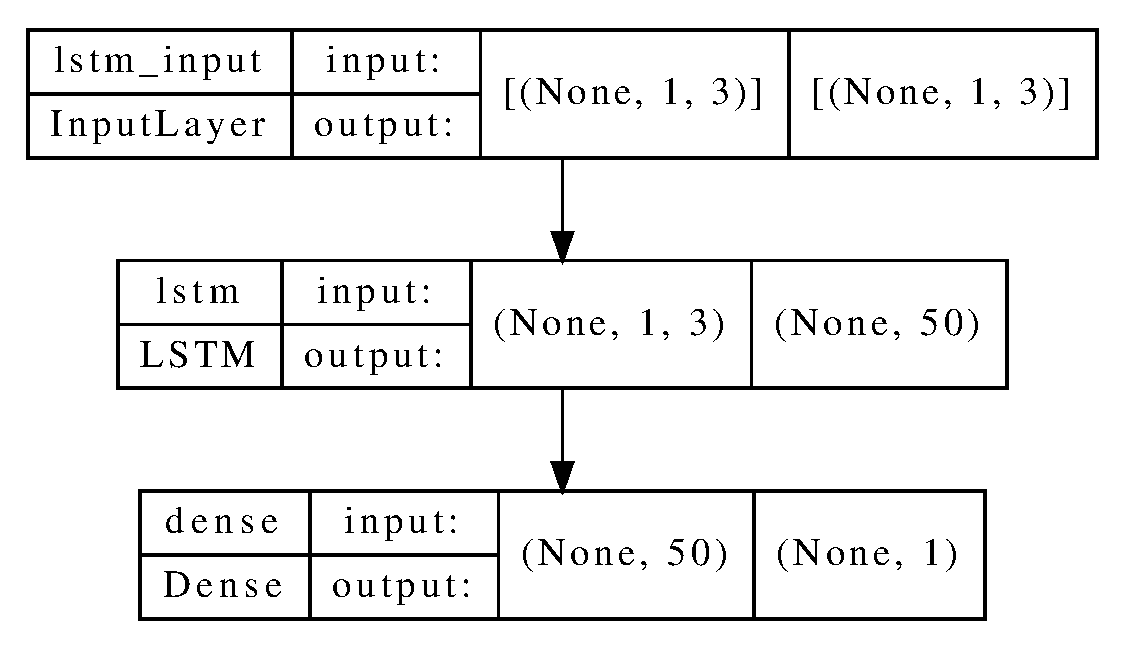
\includegraphics[width=0.8\textwidth]{LSTM.eps}
    \end{center}
    \caption{本文所使用的LSTM模型结构}
    \label{fig:my_model_arch}
\end{figure}

\subsection{模型训练}
\label{sec:model_train}
本文在模型训练过程中将学习率设置为0.01,batch size设置为64,并使用Adam优化器。另外,使用平均绝对误差(Mean Absolute Error,MAE)作为损失函数。MAE的定义如公式(\ref{eq:MAE})所示。
\begin{equation}
    MAE=\frac{1}{N}\sum_{i=1}^N|y_p-y_g|
    \label{eq:MAE}
\end{equation}
其中,$N$表示总样本数目,$y_p$与$y_g$分别表示模型预测距离以及真实距离。模型训练过程中模型在训练集以及测试集的损失变化情况如图\ref{fig:train_MAE_loss}所示。
\begin{figure}[htbp]
    \begin{center}
        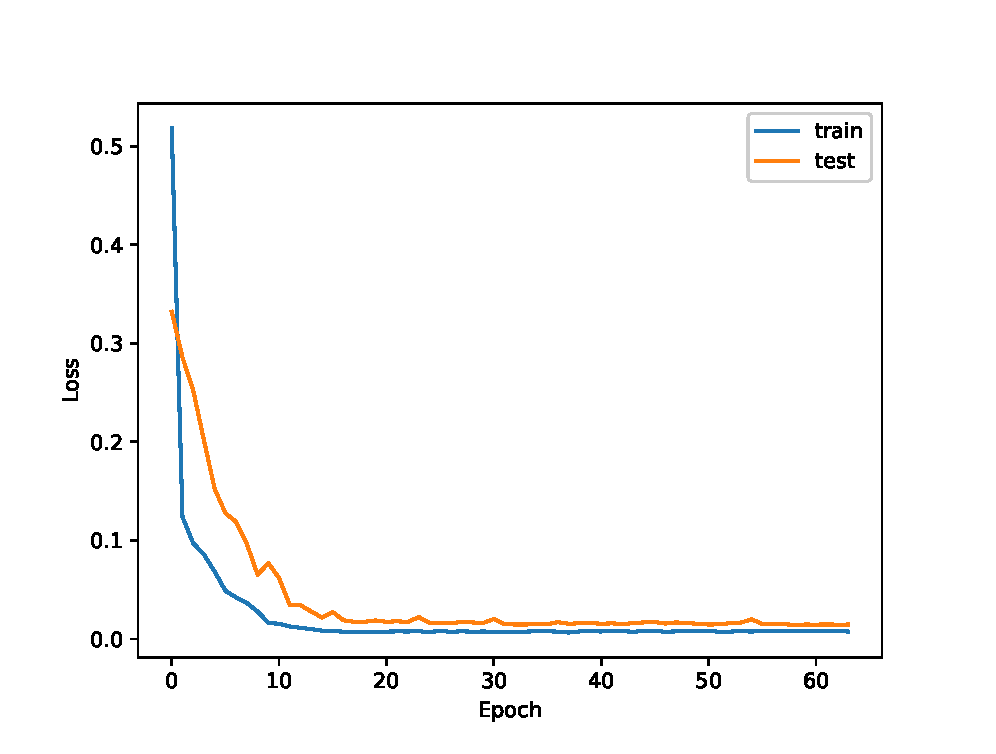
\includegraphics[width=0.8\textwidth,trim={0 10 0 10},clip]{train_loss.eps}
    \end{center}
    \caption{平均绝对误差(MAE)}
    \label{fig:train_MAE_loss}
\end{figure}

紧接着,在模型训练完成后,以RMSE作为评价指标,并统计模型的最大误差、最小误差与平均误差,从而对模型的有效性进行评估。RMSE计算公式如(\ref{eq:RMSE})所示。
\begin{equation}
    RMSE=\frac{1}{N}\sqrt{\sum_{i=1}^N(y_p-y_g)^2}
    \label{eq:RMSE}
\end{equation}
其中,$N$表示总测试样本数目,$y_p$与$y_g$分别表示模型输出的预测距离与真实距离。所得出的评估结果如表(\ref{tab:metrics})所示。

\begin{table}
    \begin{center}
    \begin{tabular}{ccl}
        \toprule
        评估指标 & 值 \\
        \midrule
        RMSE & 0.072 \\
        min error & -0.000957(m) \\
        max error & 1.043058(m) \\
        average error & 0.070112(m) \\
        \bottomrule
    \end{tabular}
    \end{center}
    \caption{模型测试后统计得出的各评估指标}
    \label{tab:metrics}
\end{table}

另外,为了直观呈现模型的有效性,图\ref{fig:model_eval}展示了测试集上预测距离值与真实距离值的曲线图。
\begin{figure}[htbp]
    \begin{center}
        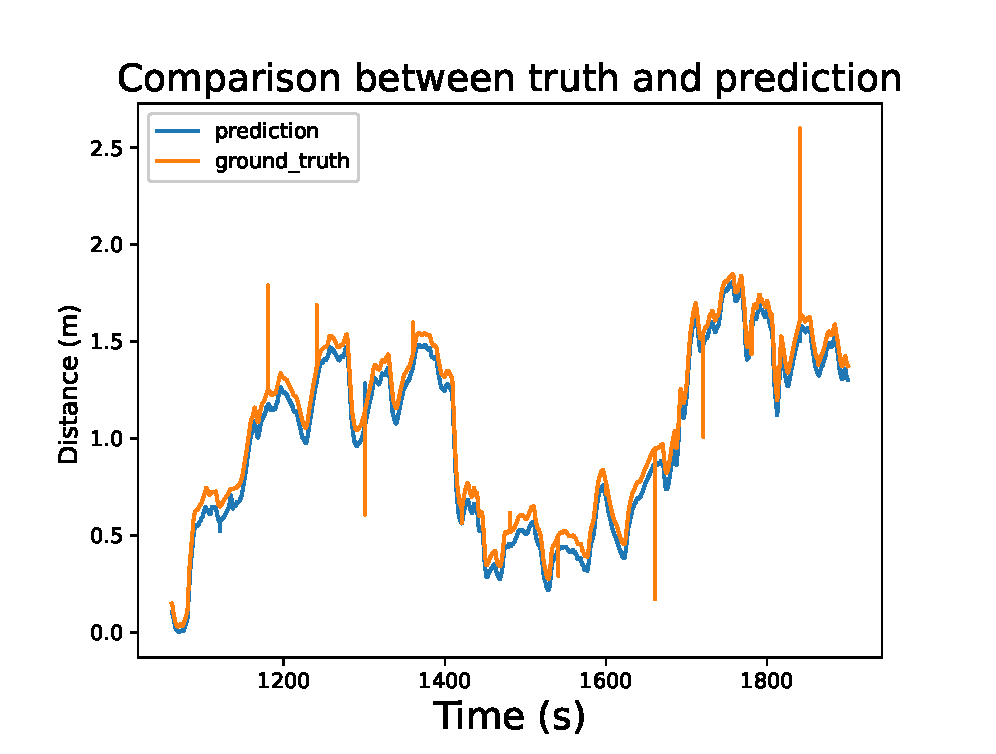
\includegraphics[width=0.8\textwidth,trim={0 0 10 0},clip]{model_eval.eps}
    \end{center}
    \caption{预测距离值与真实距离值对比}
    \label{fig:model_eval}
\end{figure}
从表(\ref{tab:metrics})以及图\ref{fig:model_eval}可以看出,模型的预测精确度较高,可以较好地实现GNSS位置欺骗攻击检测的目的。

\subsection{GNSS位置欺骗攻击检测}
本文所采取的欺骗攻击检测方法,是通过比对上述模型的预测行驶距离与实际行驶距离来实现的。若两者间的差值大于误差阈值,则认为此时目标车辆受到了欺骗。检测算法伪代码见算法\ref{algo:dectection}。\ref{sec:model_train}中定义欺骗阈值$\gamma=\epsilon_{GNSS}+\epsilon_{LSTM}$。另外,由\ref{sec:model_train}可得知,模型的平均预测误差为0.070112m;同时,由\cite{kaplan2005understanding}可知,目前常用的GNSS定位技术误差可认为是10m。因此,有$\gamma=10+0.070112=10.070112(m)$。

\begin{algorithm}
    \KwIn{来自CAN的车速$v$, 来自IMU的前向加速度$a_{forward}$, 转向角$\omega$,来自GNSS模块的实际行驶距离$dis_{truth}$,行驶距离预测模型$M$,欺骗阈值$\gamma$}
    \KwOut{表示是否受到欺骗的布尔值$spoofed$}
    $dis_{predict}=M(v, a_{forward}, \omega)$\;
    \eIf {$\|dis_{predict}-dis_{truth}\|>\gamma$}
    {
        $spoofed\leftarrow True$\;
    }{
        $spoofed\leftarrow False$\;
    }
    \KwRet{$spoofed$}\;
    \caption{GNSS位置欺骗攻击检测算法}
    \label{algo:dectection}
\end{algorithm}

\subsection{本章小结}
本章主要介绍了基于LSTM的智能网联汽车GNSS位置欺骗攻击检测算法的基本思路、模型结构以及训练细节。同时通过MAE与RMSE说明了模型的有效性。

	\section{GNSS位置欺骗攻击功能安全应急策略}
\subsection{智能网联汽车GNSS功能与功能安全风险项分析}
要设计功能安全应急策略,首先要分析可能会遇到安全风险的功能有哪些。在智能网联汽车中,GNSS模块主要负责为车辆自动驾驶算法模块提供当前位置、速度、转向角,从而保证自动驾驶算法可以及时规划路线。当该功能因受到GNSS位置欺骗攻击而出现故障时,有可能会出现不同的功能安全风险。具体可见表\ref{tab:gnss_shixiao}。
\begin{table}[]
    \begin{center}
    \begin{tabular}{|c|c|}
    \hline
    GNSS模块功能 & \multicolumn{1}{c|}{功能安全风险}\\ \hline
    \multirow{2}{*}{\begin{tabular}[c]{@{}c@{}}为车辆自动驾驶算法\\ 提供当前位置、速度、转向角\end{tabular}} & \begin{tabular}[c]{@{}c@{}}车辆远离正确规划路线,\\ 但车辆目前所处环境较为安全\\ (周围无障碍物、行人等)\end{tabular}     \\ \cline{2-2}
 & \begin{tabular}[c]{@{}c@{}}车辆远离正确规划路线,\\ 且车辆目前所处环境复杂\\ (山路、窄路、雨天、湖泊或河流旁等)\end{tabular} \\ \hline
    \end{tabular}
    \end{center}
    \caption{GNSS模块在受到欺骗后可能遇到的功能安全风险}
    \label{tab:gnss_shixiao}
\end{table}
\subsection{应用HARA方法划分风险等级}
\paragraph{车辆远离正确规划路线,但车辆所处环境较为安全}
对于该风险,由于车辆所处的环境比较安全,周围没有明显障碍物或行人,因此,发生交通事故的可能性会相对较低,严重度可以认为是S1。对于暴露度,由于当前智能网联汽车多属于消费级汽车,所处环境一般位于城市道路、小区道路等,处于空旷环境的概率较小,因此E因子应被划分为E2;最后,对于C因子,由于此时所处环境较为简单空旷,因此驾驶人一般可以有足够的时间接管汽车并调整方向,故C因子应该被划分为C1。对照表\ref{tab:ASIL},该功能安全风险的等级为QM。
\paragraph{车辆远离正确规划路线,且车辆所处环境复杂}
对于该风险,由于车辆所处环境比较复杂,周围有明显障碍物或行人,因此,相比在安全环境中,此时会更容易发生交通事故,故严重度应该被分类为S3。如上文所述,当前智能网联汽车多处于城市道路等复杂环境,但也会有处于空旷地区等简单环境的情况。因此,可以认为E因子为E3。最后,由于此时所处环境复杂,一旦发生功能失效,司机往往较难在事故发生前接管并控制车辆脱离风险,因此,认为C因子为C3。综上,对照表\ref{tab:ASIL},该功能安全风险的等级为C。

上文对具体功能所涉及到的S、E、C因子以及ASIL进行了划分。具体见表\ref{tab:gnss_sec_asil_zongjie}。
\begin{table}
\begin{center}
    \begin{tabular}{ccccc}
    \hline
    功能安全风险                                                            & 严重度 & 暴露度 & 可控性 & ASIL \\ \hline
    \begin{tabular}[c]{@{}c@{}}车辆远离规划路线,\\ 但车辆目前所处环境较为安全\end{tabular} & S1  & E2  & C1  & QM   \\ \hline
    \begin{tabular}[c]{@{}c@{}}车辆远离规划路线,\\ 且车辆目前所处环境复杂\end{tabular}   & S3  & E3  & C3  & C    \\ \hline
    \end{tabular}
\end{center}
\caption{对GNSS模块受到位置欺骗攻击后可能会遇到的功能安全风险使用HARA方法分析,得到的S、E、C因子以及ASIL}
\label{tab:gnss_sec_asil_zongjie}
\end{table}

\subsection{设计应急策略}
对于上述两种功能安全风险,本文分别提出以下功能安全应急策略:
\paragraph{车辆远离规划路线,但车辆目前所处环境较为安全}
该风险的ASIL为QM。若车辆面临该风险,则尽可能调低GNSS模块在汽车定位算法中的权重,同时提高其他模块,如IMU、LiDAR、RADAR的权重,GNSS模块同时应根据其他传感器的定位结果恢复正常功能;另外,车辆进入辅助驾驶模式,由驾驶人接管车辆驾驶,自动驾驶模块仅为驾驶人提供有限的、必要的辅助驾驶功能(如制动辅助)。
\paragraph{车辆原理规划路线,且车辆目前所处环境复杂}
该风险的ASIL为C。若车辆面临该风险,则自动驾驶模块应立即将驾驶权交由驾驶人接管。同时,GNSS模块应借助IMU、LiDAR、RARAR等传感器得出的定位结果尽可能恢复正常功能。
\subsection{本章小结}
本章主要对智能网联汽车在GNSS模块受到位置欺骗攻击的情况下有可能面临的功能安全风险进行了分析,并使用HARA方法划分了对应的风险等级。同时,在风险等级的基础上,针对两种功能安全风险,提出了对应的应急策略。

	\section{实验与结果分析}
\subsection{训练数据集概述与数据处理}
\subsection{攻击生成}
\subsection{基于CARLA的仿真实验验证}
\subsection{本章小结}

	\section{结论与展望}
\subsection{结论}
\subsection{进一步研究工作}

	\include{data/chapter07}


	%参考文献
    \kaishu
	\bibliographystyle{apalike}
	\addcontentsline{toc}{section}{参考文献} %向目录中添加条目,以章/section的名义
	\bibliography{main}


	%致谢与英文摘要
	\fangsong
	\newpage

\section*{\centerline{\heiti\zihao{-4}{致谢}}}
\addcontentsline{toc}{section}{致谢}

\vspace{5bp}

\vspace{5bp}

\vspace{5bp}

\vspace{5bp}

\vspace{5bp}

	\newpage

\centerline{\fangsong\bf\zihao{-2}{Research on Content-Aware Collaborative Filtering }}

\addcontentsline{toc}{section}{Abstract(Key words)}

\vskip 20bp

\hspace{4bp} {\zihao{-4}\textbf{【 Abstract】}}
With the booming development of machine learning, data mining and other technologies, various emerging technologies are being created. This includes intelligent connected cars. Smart Internet-connected vehicles are different from traditional cars in that they are equipped with various sensors and actuators, as well as combined with modern communication and interconnection technologies, which can realize information exchange between vehicles, vehicles and people, and vehicles and roads. However, the GNSS location spoofing problem associated with intelligent connected cars also frequently plagues major manufacturers and researchers. Therefore, this paper focuses on the detection of GNSS position spoofing attacks on intelligent connected cars and the corresponding functional safety contingency strategies. The main work of this paper can be summarized as the following three points.
\begin{enumerate}
    \item For GNSS position spoofing attacks on intelligent connected cars, an algorithm that can effectively implement attack detection is designed and implemented based on LSTM networks in machine learning, using publicly available datasets to build a training set. The data needed to train the LSTM network are velocity, steering angle, forward acceleration, and the distance the vehicle moves between adjacent time stamps. In this paper, the GNSS location point data in the original data are converted into distances by using the Haverson's great circle formula.
    \item The spoofing dataset was obtained by modifying part of the data in the public dataset, and experiments were conducted with this as the test set. The experimental results show that the algorithm designed in this paper can effectively detect GNSS location spoofing attacks against intelligent connected cars.
    \item Based on the ISO 26262 standard, the functional safety risks that intelligent connected vehicles may face in the case of GNSS location spoofing attacks are analyzed using the HARA method, and the corresponding risk levels are also classified, and suitable contingency strategies are designed. Thus, the linkage of algorithm detection and contingency strategy is realized.
\end{enumerate}
In summary, this paper designs a location spoofing attack detection algorithm based on LSTM technology and ISO 26262 standard for the GNSS module of intelligent connected cars, and also designs a corresponding functional safety contingency strategy. The detection algorithm can work effectively, but there is still room for improvement in the scene refinement. The GNSS positioning error in different scenarios can be obtained later by collecting data from real vehicles, so as to refine the detection performance in different driving scenarios.

\vskip 10bp

\hspace{5bp}{\zihao{-4}\textbf{【 Keywords】}}
intelligent Connected Vehicle; GNSS; Functional Safety; LSTM


\vskip 20bp

\begin{flushright}
	\kaishu 指导教师:\ 肖志娇 \hspace{3cm}{ }
\end{flushright}

\label{lastpage}%%%%显示总页数

\end{document}
